\documentclass[11pt,a4paper]{article}
\usepackage[T1]{fontenc}
\usepackage[utf8]{inputenc}
\usepackage{amsmath}
\usepackage{mathpazo}
\usepackage[scaled=0.9]{helvet}
\usepackage{courier}
\usepackage[margin=2.3cm]{geometry}
\usepackage{microtype}
\usepackage{xcolor}
\usepackage{listings}
\usepackage{booktabs}
\usepackage{tabularx}
\usepackage{enumitem}
\usepackage{graphicx}
\usepackage{caption}
\usepackage{array}
\usepackage{float}
\newcolumntype{Y}{>{\raggedright\arraybackslash}X}
\usepackage{tikz}
\usetikzlibrary{arrows.meta,positioning,fit}
\usepackage[hidelinks]{hyperref}

\definecolor{kw}{HTML}{1F4E9A}
\definecolor{cm}{HTML}{6A737D}
\definecolor{bg}{HTML}{F6F8FA}
\lstset{language=Java, basicstyle=\ttfamily\fontsize{7.9}{9.6}\selectfont, keywordstyle=\color{kw}\bfseries,
  commentstyle=\color{cm}\itshape, backgroundcolor=\color{bg}, frame=single, rulecolor=\color{bg},
  columns=fullflexible, keepspaces=true, showstringspaces=false, aboveskip=6pt, belowskip=6pt,
  xleftmargin=4pt, xrightmargin=4pt}
\setlist{itemsep=2pt,topsep=4pt}
\setlength{\parskip}{4pt}
\setlength{\parindent}{0pt}
\newcommand{\code}[1]{\texttt{\hyphenchar\font=-1 #1}}
\sloppy

\title{\textbf{FSStat} \\[2pt] \large Assignment \#02 --- Concurrent and Distributed Programming}
\author{Eduard Toni Alexandru}
\date{a.y. 2025--2026 \quad$\cdot$\quad Java 21, Vert.x 5.0.10, RxJava 3.1.8}

\begin{document}
\maketitle

\section{Analysis}

\subsection{Requirements}

\begin{table}[h]
\centering\small
\begin{tabularx}{\textwidth}{@{}lY@{}}
\toprule
\textbf{Id} & \textbf{Requirement} \\
\midrule
R1 & \code{getFSReport(D, MaxFS, NB)} is \emph{asynchronous}: the caller is not blocked and obtains the
     report \code{R} when it is ready. \\
R2 & \code{R} contains the total number of files in \code{D}, recursively. \\
R3 & \code{R} contains the distribution of file sizes over $NB+1$ bands: $NB$ equal intervals of
     $[0, MaxFS]$ and one band for files bigger than \code{MaxFS}. \\
R4 & An example program shows the use of the library (one per version). \\
R5 (ext.) & The generation of a report can be \emph{stopped}. \\
R6 (ext.) & Partial statistics are \emph{dynamically} available while the report is being generated,
     e.g.\ to show them in a GUI with start/stop buttons. \\
R7 & Each version follows the discipline of its approach (event loop, Rx, virtual threads) and does not
     reuse code when this would compromise that discipline. \\
\bottomrule
\end{tabularx}
\caption{Requirements (from the assignment text).}\label{tab:req}
\end{table}

Some points left open by the text were fixed as follows. The band of a file of size $s$ is
\[
  band(s) = \begin{cases} NB & s > MaxFS\\ \min\left(\left\lfloor s\cdot NB / MaxFS \right\rfloor,\ NB-1\right) & \text{otherwise}\end{cases}
\]
so a file of exactly \code{MaxFS} bytes falls in the last regular band (the interval is closed) and no
truncation of the band width occurs when \code{MaxFS} is not a multiple of \code{NB}. Only regular files
are counted; symbolic links are not followed (otherwise a link to an ancestor would create an infinite
tree); unreadable files and directories are skipped, because a single permission error must not
abort a report on a whole file system. An invalid root or invalid parameters make the whole
request fail.

\subsection{Structure of the problem}

The computation follows the shape of the directory tree. For a directory $d$ with files $f_1..f_k$ and
sub-directories $d_1..d_m$:
\[
  R(d) \;=\; \bigoplus_{i=1}^{k} \mathit{one}(f_i) \;\oplus\; \bigoplus_{j=1}^{m} R(d_j)
\]
where $\mathit{one}(f)$ is a report with a single file in band $band(size(f))$ and $\oplus$ sums
the counters band by band. Two properties of $\oplus$ drive the whole design:
\begin{itemize}
  \item it is \textbf{associative and commutative}, with the empty report as neutral element: partial
        results can be combined in \emph{any order} and grouped in \emph{any way}, so the sub-trees
        can be explored concurrently and their results merged as soon as they are available;
  \item it works on \textbf{small immutable values} ($NB+2$ numbers): merging is cheap and partial
        reports can be passed between activities without copying large data.
\end{itemize}
This is a classic \emph{divide and conquer} / map-reduce pattern: \emph{map} = list a directory and
read the attributes of each entry (I/O), \emph{reduce} = $\oplus$. In our code the value is the record
\code{FSReport}, whose \code{empty}, \code{addFile} and \code{merge} methods implement the neutral
element, $\mathit{one}$ and $\oplus$.

\subsection{Concurrency aspects}

\begin{itemize}
  \item \textbf{I/O-bound work of unknown size.} Almost all the time is spent waiting for the file
        system. Concurrency is useful to have many I/O requests in flight, not to use many cores. The
        shape and size of the tree are discovered only while exploring it, so the number of tasks is
        not known in advance and new work is generated dynamically.
  \item \textbf{Termination detection.} The report is complete only when every directory at any depth
        has been processed. With dynamically generated work, completion has to be propagated
        bottom-up: a directory is done when all its entries are done.
  \item \textbf{Aggregation and shared state.} Thanks to the properties of $\oplus$, the base problem
        can be solved with \emph{no shared mutable state}: each sub-tree returns its own report and
        the parent merges them. Shared state is needed only by the extension (R6), because someone
        must be able to observe the partial result \emph{while} it is being built.
  \item \textbf{Observer vs.\ workers} (R6). Partial results are written by the scanning activities
        and read by an observer: the two must not race (no torn or inconsistent snapshots), and the
        observer must not be flooded (one update per file would saturate the GUI: a few updates per
        second are enough).
  \item \textbf{Cancellation} (R5). A stop request is asynchronous with respect to the scan: it must
        reach activities that are already running, stop the generation of new work, and leave the
        system in a consistent state: a final notification is delivered, no update arrives after it,
        and a new scan can be started without interference from the old one.
  \item \textbf{GUI thread confinement.} Swing components may be touched only by the Event
        Dispatch Thread (EDT). Results produced by library threads must be handed over to the EDT, and
        the EDT must never block waiting for the library.
  \item \textbf{Bounding resources.} Every listing and every attribute read is a pending I/O
        operation; exploring all sub-trees at once is possible, but each approach has its own way to
        absorb or limit this (worker pool, schedulers, virtual threads).
\end{itemize}

\subsection{Actors and interactions}

Abstracting from the technology, the interactive application involves three kinds of actors:
\begin{itemize}
  \item the \textbf{user / GUI} (EDT), which issues \emph{start} and \emph{stop} commands and displays
        reports;
  \item the \textbf{scan}, a dynamic set of activities exploring the tree and producing partial results;
  \item an \textbf{update source}, which periodically turns the current partial result into an update
        for the GUI (this is what limits the update rate).
\end{itemize}
The \emph{start} command creates a new scan; \emph{stop} and the natural end of the scan both lead to a
single final notification (\emph{completed}, \emph{stopped} or \emph{failed}). Each version maps these
actors onto its own concepts; the mapping is the core of the design (Section~\ref{sec:design}).

\section{Design}\label{sec:design}

\subsection{Overall architecture and shared parts}

The code is organised in three layers (Figure~\ref{fig:arch}):
\begin{itemize}
  \item \code{lib.*}: the three versions of the library, one package each;
  \item \code{app.*}: for each version, an example program for the base library (\code{...CLI}) and a
        GUI program for the extension (\code{...GUI}), with a version-specific controller;
  \item \code{view}: a Swing GUI (\code{FSStatView}) shared by the three GUI programs.
\end{itemize}

\begin{figure}[H]
\centering
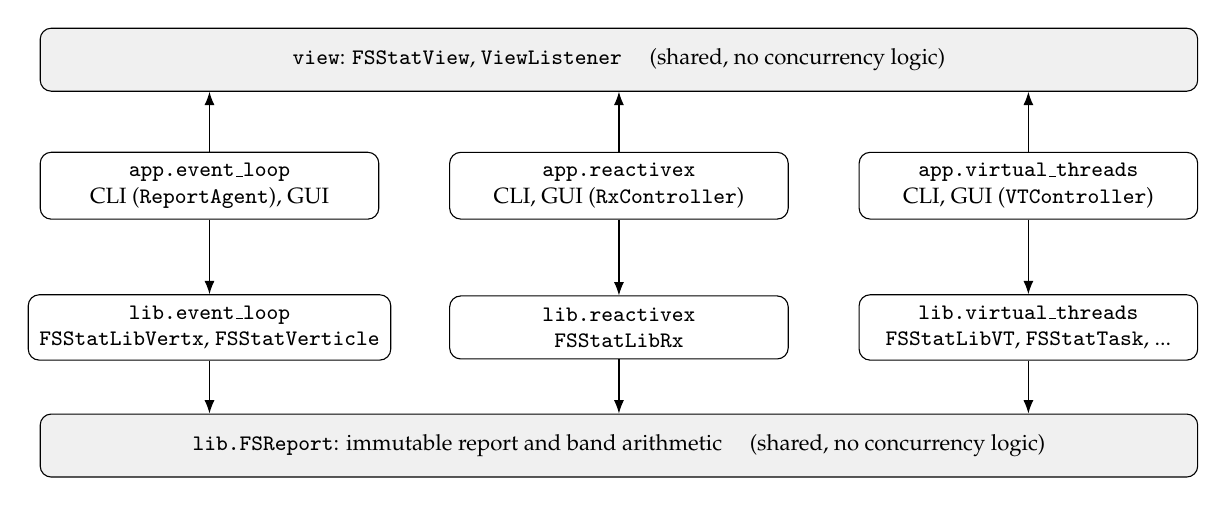
\begin{tikzpicture}[every node/.style={font=\footnotesize},
  pkg/.style={draw, rounded corners, align=center, minimum height=0.8cm, inner sep=4pt},
  sh/.style={pkg, fill=black!6}]
  \node[pkg, minimum width=4.3cm] (l1) at (0,0) {\code{lib.event\_loop}\\\code{FSStatLibVertx}, \code{FSStatVerticle}};
  \node[pkg, minimum width=4.3cm] (l2) at (5.2,0) {\code{lib.reactivex}\\\code{FSStatLibRx}};
  \node[pkg, minimum width=4.3cm] (l3) at (10.4,0) {\code{lib.virtual\_threads}\\\code{FSStatLibVT}, \code{FSStatTask}, ...};
  \node[pkg, minimum width=4.3cm] (a1) at (0,1.8) {\code{app.event\_loop}\\CLI (\code{ReportAgent}), GUI};
  \node[pkg, minimum width=4.3cm] (a2) at (5.2,1.8) {\code{app.reactivex}\\CLI, GUI (\code{RxController})};
  \node[pkg, minimum width=4.3cm] (a3) at (10.4,1.8) {\code{app.virtual\_threads}\\CLI, GUI (\code{VTController})};
  \node[sh, minimum width=14.7cm] (v) at (5.2,3.4) {\code{view}: \code{FSStatView}, \code{ViewListener} \quad (shared, no concurrency logic)};
  \node[sh, minimum width=14.7cm] (r) at (5.2,-1.5) {\code{lib.FSReport}: immutable report and band arithmetic \quad (shared, no concurrency logic)};
  \foreach \i in {1,2,3} { \draw[-{Latex}] (a\i) -- (l\i); \draw[-{Latex}] (a\i) -- (a\i |- v.south); \draw[-{Latex}] (l\i) -- (l\i |- r.north); }
\end{tikzpicture}
\caption{Packages and dependencies. Grey parts are shared by the three versions.}\label{fig:arch}
\end{figure}

Only two parts are shared, and both are free of concurrency logic, so sharing them does not affect the
discipline of any version (R7):
\begin{itemize}
  \item \code{FSReport}, the immutable value of the analysis ($\oplus$ and the band function): every
        version needs exactly the same arithmetic, and an immutable value can be passed between threads
        safely;
  \item the Swing view, built as in the MVC examples of the course: it forwards user commands to a
        \code{ViewListener} (the controller) and exposes \code{showReport} and \code{showFinished},
        which can be called from any thread because they only schedule the update on the EDT with
        \code{SwingUtilities.invokeLater}.
\end{itemize}
Conversely, there is deliberately \emph{no common library interface}. A single interface would force
the same shape (e.g.\ a callback-based method) on all versions, while each approach has its own
abstraction for ``a result that will be available later'': a Vert.x \code{Future}, an Rx \code{Single},
a blocking \code{Future.get()} on a virtual thread. The same holds for the extension: an event-bus
protocol, a \code{Flowable} of partial reports, a listener called by virtual threads
(Table~\ref{tab:api}). For the same reason each version has its own controller.

\begin{table}[H]
\centering\small
\begin{tabularx}{\textwidth}{@{}lYY@{}}
\toprule
 & \textbf{Base (R1--R3)} & \textbf{Extension (R5, R6)} \\
\midrule
Event loop & \code{Future<FSReport> getFSReport(...)}, to be called from a verticle &
  \code{FSStatVerticle}: updates and outcome published on the event bus; stop = a message \\
Reactive & \code{Single<FSReport> getFSReport(...)} &
  \code{Flowable<FSReport> getFSReportStream(...)}: stream of partial reports; stop = \code{dispose()} \\
Virtual threads & \code{Future<FSReport> getFSReport(...)} computed by a virtual thread
  (plus the synchronous \code{computeFSReport}) &
  \code{FSStatTask}: an \code{FSStatListener} is notified (\code{onUpdate}, \code{onCompleted}, \code{onStopped}, \code{onFailed}); cooperative \code{stop()} \\
\bottomrule
\end{tabularx}
\caption{API of the three versions.}\label{tab:api}
\end{table}

\subsection{Event-loop version: components}

In Vert.x the unit of concurrency is the \emph{verticle}: an event loop that owns its state and
reacts to events (I/O completions, timers, messages) one at a time. Two rules shape the design:
(i) the continuations of a Vert.x future run on the event loop (context) of whoever called the
asynchronous operation; (ii) different verticles never share state, they communicate through the
event bus. Hence every piece of logic is placed \emph{inside} a verticle.

\begin{figure}[H]
\centering
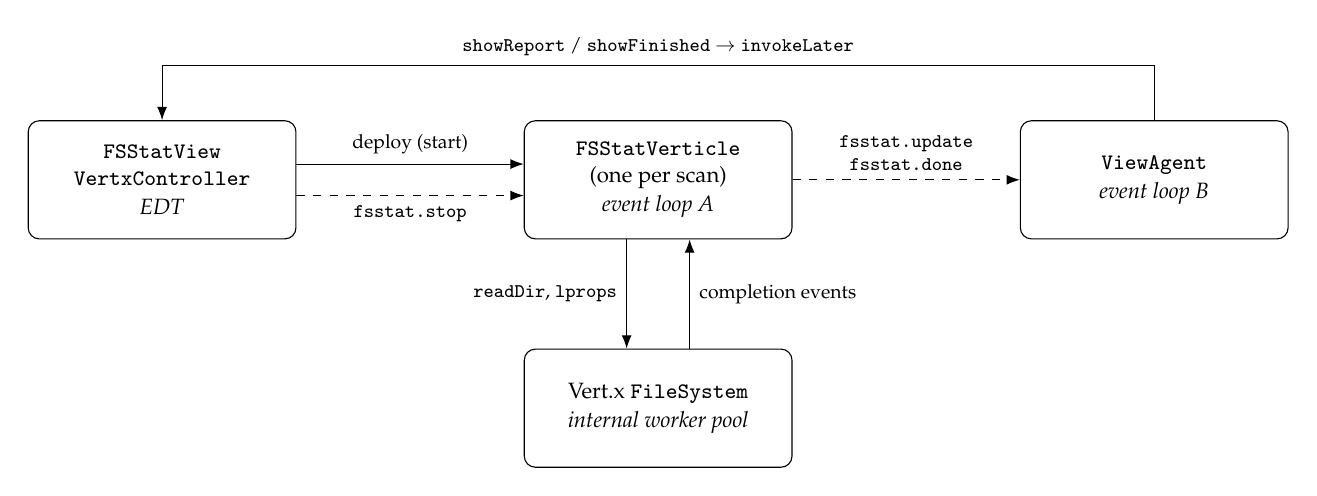
\begin{tikzpicture}[every node/.style={font=\footnotesize},
  box/.style={draw, rounded corners, minimum width=3.4cm, minimum height=1.5cm, align=center},
  lab/.style={font=\scriptsize}]
  \node[box] (view) at (0,0) {\code{FSStatView}\\\code{VertxController}\\[1pt]\textit{EDT}};
  \node[box] (scan) at (6.3,0) {\code{FSStatVerticle}\\(one per scan)\\[1pt]\textit{event loop A}};
  \node[box] (agent) at (12.6,0) {\code{ViewAgent}\\[1pt]\textit{event loop B}};
  \node[box] (fs) at (6.3,-2.9) {Vert.x \code{FileSystem}\\[1pt]\textit{internal worker pool}};
  \draw[-{Latex}] ([yshift=2mm]view.east) -- node[above, lab]{deploy (start)} ([yshift=2mm]scan.west);
  \draw[-{Latex}, dashed] ([yshift=-2mm]view.east) -- node[below, lab]{\code{fsstat.stop}} ([yshift=-2mm]scan.west);
  \draw[-{Latex}, dashed] (scan) -- node[above, lab, align=center]{\code{fsstat.update}\\\code{fsstat.done}} (agent);
  \draw[-{Latex}] (agent.north) -- ++(0,0.7) -| node[pos=0.25, above, lab]{\code{showReport} / \code{showFinished} $\to$ \code{invokeLater}} (view.north);
  \draw[-{Latex}] ([xshift=-4mm]scan.south) -- node[left, lab]{\code{readDir}, \code{lprops}} ([xshift=-4mm]fs.north);
  \draw[-{Latex}] ([xshift=4mm]fs.north) -- node[right, lab]{completion events} ([xshift=4mm]scan.south);
\end{tikzpicture}
\caption{Event-loop version, GUI program. Dashed arrows are event-bus messages.}\label{fig:vertx}
\end{figure}

\begin{itemize}
  \item \textbf{\code{FSStatLibVertx}} (base library) is a passive object: \code{getFSReport} builds a
        composition of futures and returns immediately. Since continuations run on the caller's
        event loop, the whole scan is executed by one thread and needs no synchronization, but only if
        the method is called \emph{from an event loop}.
  \item \textbf{\code{ReportAgent}} (CLI example) exists for exactly that reason. The \code{main}
        thread is not an event loop: if it called the library directly, the operations would be bound
        to contexts that Vert.x creates implicitly for a foreign thread, and the single-thread
        guarantee would rest on an implementation detail rather than on the design. So \code{main}
        only creates Vert.x and deploys \code{ReportAgent}, a verticle whose \code{start()} calls
        \code{getFSReport} and prints the result when the future completes, as in the lab examples
        where all the logic lives in a verticle. When the report is ready the agent closes Vert.x
        (scheduled with \code{runOnContext}, so that it happens after \code{start()} has returned,
        also when the future fails immediately).
  \item \textbf{\code{FSStatVerticle}} (extension) is the scan as an \emph{active} component. The
        extension needs state that lives during the scan and changes over time: counters, a stopped
        flag, a periodic timer, a subscription to stop messages. Putting this state in a verticle
        confines it to one event loop, so plain fields are enough. One verticle is deployed for each
        scan and it undeploys itself at the end: a new scan never shares state with an old one, and
        the lifecycle of the scan coincides with the lifecycle of the verticle.
  \item \textbf{\code{VertxController}} translates GUI commands into Vert.x actions:
        \emph{start} = deploy a new \code{FSStatVerticle}, \emph{stop} = publish on \code{fsstat.stop}.
        It deliberately keeps no reference to the running verticle (not even its deployment id, which
        would be written by an event loop and read by the EDT): the only link between the EDT and the
        scan is message passing.
  \item \textbf{\code{ViewAgent}} receives the messages of the scan and forwards them to the view.
        It is a verticle, rather than a set of consumers registered by \code{main}, for the same
        reason as \code{ReportAgent}: by construction, the handlers of \code{fsstat.update} and
        \code{fsstat.done} run on one known event loop, one at a time, and messages sent by the
        scanning verticle are handled in the order they were sent, so a late update cannot overwrite
        the final report. It also follows the lab examples (event-bus consumers registered in a
        verticle), and it is deployed before the window is shown, so the consumers exist before the
        first scan can start. \code{ViewAgent} is the bridge between the event-loop world and the EDT.
\end{itemize}

\subsection{Reactive version: components}

In Rx the unit of design is the \emph{stream}, and concurrency is a property of the pipeline
(schedulers), not of the components. The library therefore only \emph{describes} computations; they
run when someone subscribes, and stop when the subscription is disposed.

\begin{figure}[H]
\centering
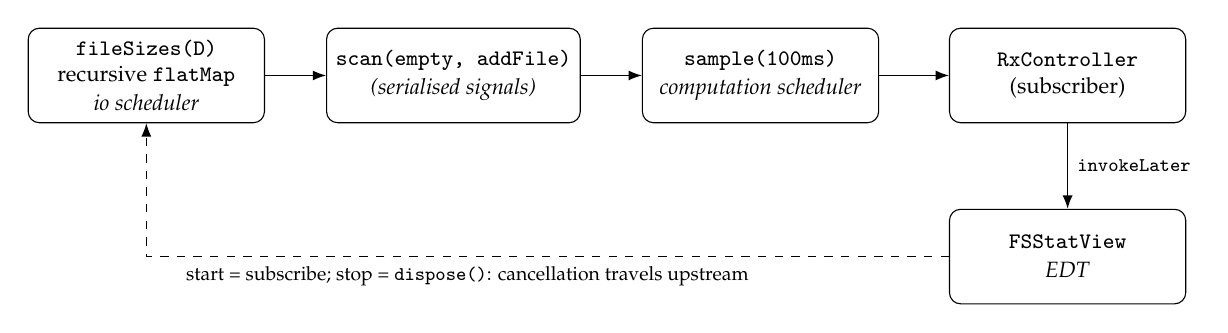
\begin{tikzpicture}[every node/.style={font=\footnotesize},
  op/.style={draw, rounded corners, minimum width=3.0cm, minimum height=1.2cm, align=center},
  lab/.style={font=\scriptsize}]
  \node[op] (src) at (0,0) {\code{fileSizes(D)}\\recursive \code{flatMap}\\[1pt]\textit{io scheduler}};
  \node[op] (scan) at (3.9,0) {\code{scan(empty, addFile)}\\[1pt]\textit{(serialised signals)}};
  \node[op] (sample) at (7.8,0) {\code{sample(100ms)}\\[1pt]\textit{computation scheduler}};
  \node[op] (sub) at (11.7,0) {\code{RxController}\\(subscriber)};
  \node[op] (view) at (11.7,-2.3) {\code{FSStatView}\\[1pt]\textit{EDT}};
  \draw[-{Latex}] (src) -- (scan); \draw[-{Latex}] (scan) -- (sample); \draw[-{Latex}] (sample) -- (sub);
  \draw[-{Latex}] (sub) -- node[right, lab]{\code{invokeLater}} (view);
  \draw[-{Latex}, dashed] (view.west) -| node[pos=0.3, below, lab]{start = subscribe;\ stop = \code{dispose()}: cancellation travels upstream} (src.south);
\end{tikzpicture}
\caption{Reactive version, GUI program: the interactive pipeline.}\label{fig:rx}
\end{figure}

\begin{itemize}
  \item \textbf{\code{FSStatLibRx}} is a factory of cold streams with no threads and no state of its
        own. Its core is \code{fileSizes(D)}, the stream of the sizes of all the regular files under
        \code{D}; the two public methods are folds over it: \code{reduce} gives the final report
        (\code{Single}), \code{scan} the sequence of partial reports (\code{Flowable}). The base
        method and the extension are thus two views of the same stream, which is the reactive way to
        satisfy R6.
  \item \textbf{No agents are needed}: the role played by \code{FSStatVerticle} in Vert.x (owning the
        partial state) is played by the \code{scan} operator, whose accumulator is safe because Rx
        serialises the signals of a stream; the role of the periodic timer is played by \code{sample},
        chosen by the \emph{consumer}, which is where the desired update rate is known.
  \item \textbf{\code{RxController}} is the subscriber. It owns the \code{Disposable} of the current
        scan, used only by the EDT (start and stop are both GUI events), so it needs no
        synchronization. Errors and completion arrive as stream signals.
  \item \textbf{\code{FSStatRxCLI}} simply subscribes to the \code{Single} with
        \code{blockingSubscribe}, as in the lab examples, to keep \code{main} alive until the end.
\end{itemize}

\subsection{Virtual-threads version: components}

With virtual threads the unit of concurrency is again the thread, but threads are cheap enough to
create one per sub-directory and to block freely. The design is therefore the classic one of the
course: active entities (threads) plus passive shared entities (monitors).

\begin{figure}[H]
\centering
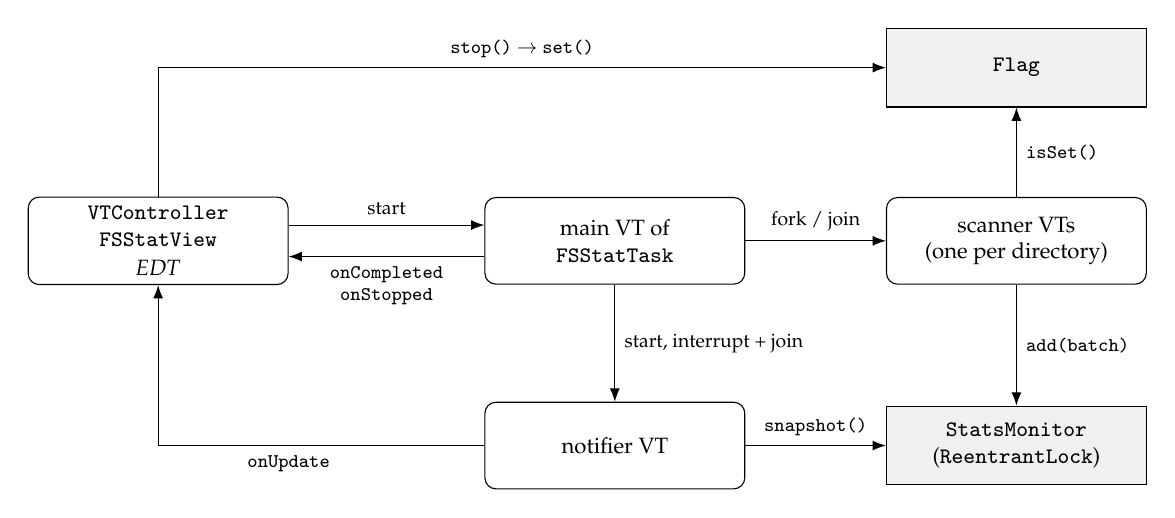
\begin{tikzpicture}[every node/.style={font=\footnotesize},
  box/.style={draw, rounded corners, minimum width=3.3cm, minimum height=1.1cm, align=center},
  mon/.style={draw, minimum width=3.3cm, minimum height=1.0cm, align=center, fill=black!6},
  lab/.style={font=\scriptsize}]
  \node[box] (ctrl) at (0,0) {\code{VTController}\\\code{FSStatView}\\[1pt]\textit{EDT}};
  \node[box] (main) at (5.8,0) {main VT of\\\code{FSStatTask}};
  \node[box] (sc) at (10.9,0) {scanner VTs\\(one per directory)};
  \node[mon] (flag) at (10.9,2.2) {\code{Flag}};
  \node[mon] (mon) at (10.9,-2.6) {\code{StatsMonitor}\\(\code{ReentrantLock})};
  \node[box] (not) at (5.8,-2.6) {notifier VT};
  \draw[-{Latex}] ([yshift=2mm]ctrl.east) -- node[above, lab]{start} ([yshift=2mm]main.west);
  \draw[-{Latex}] ([yshift=-2mm]main.west) -- node[below, lab, align=center]{\code{onCompleted}\\\code{onStopped}} ([yshift=-2mm]ctrl.east);
  \draw[-{Latex}] (main) -- node[above, lab]{fork / join} (sc);
  \draw[-{Latex}] (main) -- node[right, lab]{start, interrupt + join} (not);
  \draw[-{Latex}] (sc) -- node[right, lab]{\code{add(batch)}} (mon);
  \draw[-{Latex}] (not) -- node[above, lab]{\code{snapshot()}} (mon);
  \draw[-{Latex}] (sc) -- node[right, lab]{\code{isSet()}} (flag);
  \draw[-{Latex}] (ctrl.north) |- node[pos=0.75, above, lab]{\code{stop()} $\to$ \code{set()}} (flag.west);
  \draw[-{Latex}] (not.west) -| node[pos=0.3, below, lab]{\code{onUpdate}} (ctrl.south);
\end{tikzpicture}
\caption{Virtual-threads version, GUI program. Grey boxes are monitors; the listener calls end in
\code{invokeLater} on the view.}\label{fig:vt}
\end{figure}

\begin{itemize}
  \item \textbf{\code{FSStatLibVT}} (base) is written as sequential blocking code. One virtual thread
        per sub-directory realises the divide and conquer of the analysis: each thread counts its own
        files in a local array and returns an immutable report through a \code{Future}, so the base
        version shares nothing. \code{getFSReport} runs the computation on a new virtual thread and
        returns a \code{Future}, which is what makes the call asynchronous (R1).
  \item \textbf{\code{FSStatTask}} (extension) is an \emph{active object} representing a scan: its
        main virtual thread runs the fork/join scan, starts the notifier and, at the end, decides the
        outcome and calls the listener. One instance per scan, as for the verticle in Vert.x.
  \item \textbf{\code{StatsMonitor}} is the shared partial result that R6 requires. Writers are the
        scanner threads (in batches of 256 files, to keep contention low), the reader is the notifier.
        It is guarded by a \code{ReentrantLock}: on Java 21 a virtual thread that blocks on a
        \code{synchronized} monitor pins its carrier thread, while blocking on a
        \code{java.util.concurrent} lock simply parks the virtual thread.
  \item \textbf{The notifier} is a separate virtual thread so that the update rate (every 100\,ms) does
        not depend on the scanning threads: they only write, it only reads and pushes.
  \item \textbf{\code{Flag}} is the stop signal, the same monitor used in the course examples
        (\code{chrono\_mvc}). Cancellation is cooperative: each scanner checks it before every entry.
        Its critical sections are tiny and never block, so \code{synchronized} is harmless here.
  \item \textbf{\code{FSStatListener}} is the observer interface (as \code{CounterEventListener} in the
        lab): its methods are called by virtual threads, so \code{VTController} implements them by
        calling the thread-safe view methods.
\end{itemize}

\subsection{Cross-cutting decisions}

\begin{table}[H]
\centering\small
\begin{tabularx}{\textwidth}{@{}lYYY@{}}
\toprule
 & \textbf{Event loop} & \textbf{Reactive} & \textbf{Virtual threads} \\
\midrule
Partial state (R6) & counters in \code{FSStatVerticle}, confined to its event loop &
  \code{scan} accumulator, serialised by Rx & \code{StatsMonitor}, lock-protected \\
Who limits the rate & periodic timer of the verticle & \code{sample}, chosen by the subscriber & notifier virtual thread \\
Stop (R5) & message on \code{fsstat.stop}; \code{stopped} flag checked by callbacks; undeploy &
  \code{dispose()}: cancellation upstream & \code{Flag} checked before every entry \\
No update after the end & timer cancelled before publishing \code{done}; one event loop handles both addresses &
  Rx contract: nothing after a terminal signal or after \code{dispose} & notifier interrupted and joined before the final callback \\
Restart & new verticle per scan & new subscription per scan & new \code{FSStat\-Task} per scan \\
\bottomrule
\end{tabularx}
\caption{How each version addresses the concurrency aspects of the extension.}\label{tab:cross}
\end{table}

In all versions the GUI is updated by \emph{pushing} reports, but the library never touches Swing and
never decides how the view is drawn: it only produces reports at a bounded rate. The view methods are
the single point where control passes to the EDT, and the EDT never blocks on the library: it only
deploys/publishes, subscribes/disposes, or starts/stops a task.

\section{Event-loop version (Vert.x)}

\subsection{Base: map-reduce by composing futures}

\code{FSStatLibVertx.getFSReport} returns a \code{Future<FSReport>} and is meant to be called from a
verticle (as in the example \code{FSStatVertxCLI}). The recursion is a \emph{non-blocking}
map-reduce: each entry becomes a future (a file becomes a one-file report, a sub-directory a
recursive scan) and \code{Future.all} joins them; the merge runs in the continuation.

\begin{lstlisting}
private Future<FSReport> scanDir(String dir, FSReport empty) {
  return fs.readDir(dir).compose(entries -> {
    List<Future<FSReport>> children = entries.stream()
        .distinct().filter(e -> isChildOf(e, dir))     // drops resolved symbolic links
        .map(e -> scanEntry(e, empty)).toList();
    return Future.all(children).map(all -> {           // reduce
      FSReport report = empty;
      for (FSReport child : all.<FSReport>list()) report = report.merge(child);
      return report;
    });
  });
}
private Future<FSReport> scanEntry(String path, FSReport empty) {
  return fs.lprops(path).compose(p -> p.isDirectory() ? scanDir(path, empty)
        : Future.succeededFuture(p.isRegularFile() ? empty.addFile(p.size()) : empty))
      .otherwise(empty);                               // unreadable entry: counts nothing
}
\end{lstlisting}

\textbf{Termination} needs no counter: the future of a directory completes exactly when the futures
of all its entries have completed, so the root future completes when the whole tree is done.
\textbf{Threads}: every continuation runs on the event loop of the calling verticle, one at a time,
so there is no shared mutable state and no synchronization. The blocking file-system calls are
executed by Vert.x on its internal worker pool, and their results come back to the event loop as
events: the event loop itself never blocks. Two details: \code{readDir} returns
\emph{canonical} paths (links already resolved), so a link is recognised as an entry that is not a
direct child of the directory (or a duplicate) and is discarded; for the same reason the root is
canonicalised once with \code{executeBlocking}, the standard way to run a short blocking call.

\subsection{Extension: the scan as a verticle}

\code{FSStatVerticle} is an event loop with its own state (counters, a \code{stopped} flag, a timer):
it scans with the same future-based recursion, incrementing its counters directly, and interacts with
the rest of the application only through the event bus (Figure~\ref{fig:vertx}):


\begin{itemize}
  \item every 100\,ms a periodic timer publishes the current report on \code{fsstat.update};
  \item when the scan ends, or a message arrives on \code{fsstat.stop}, \code{finish(status)} sets
        \code{stopped}, cancels the timer, publishes the outcome (\code{completed}, \code{stopped} or
        \code{failed}) on \code{fsstat.done} and undeploys the verticle;
  \item pending callbacks check \code{stopped} and return immediately, so the remaining futures
        complete quickly and no update can follow the final message.
\end{itemize}

Since callbacks, timer and event-bus handlers are all run by the verticle's event loop, the flag and
the counters are plain fields: there is no race between the scan, the stop request and the updates.
Every scan is a new verticle instance, so a new scan never shares state with an old one; on the GUI
side \code{ViewAgent} handles updates and the final outcome in order and passes them to the EDT.

\section{Reactive version (RxJava)}

The file system is modelled as a cold stream of file sizes; the report is a fold over it.

\begin{lstlisting}
public Single<FSReport> getFSReport(Path dir, long maxFS, int nb) {
  return Single.defer(() -> fileSizes(dir)
      .reduce(FSReport.empty(maxFS, nb), FSReport::addFile));
}
public Flowable<FSReport> getFSReportStream(Path dir, long maxFS, int nb) {
  return Flowable.defer(() -> fileSizes(dir)
      .scan(FSReport.empty(maxFS, nb), FSReport::addFile));
}
private Flowable<Long> sizesIn(Path dir) {
  return Flowable.defer(() -> Flowable.fromIterable(list(dir)))
      .subscribeOn(Schedulers.io())                    // blocking listing on an I/O thread
      .flatMap(entry -> Flowable.defer(() -> {
          var attrs = Files.readAttributes(entry, BasicFileAttributes.class, NOFOLLOW_LINKS);
          if (attrs.isDirectory())   return sizesIn(entry);   // recursion: a sub-stream
          if (attrs.isRegularFile()) return Flowable.just(attrs.size());
          return Flowable.<Long>empty();
        }).onErrorResumeNext(err -> Flowable.empty()),  // unreadable entry: skipped
        MAX_CONCURRENCY);
}
\end{lstlisting}

\begin{itemize}
  \item \textbf{Concurrency.} Each directory listing is subscribed on \code{Schedulers.io()}, so
        sub-trees are explored in parallel and \code{flatMap} merges their streams. Its
        \code{maxConcurrency} argument (8) bounds the sub-streams active \emph{per directory}; since
        the bound applies at each level of the recursion, the overall concurrency is not globally
        limited to 8 (the I/O scheduler grows as needed).
  \item \textbf{Termination} is part of the protocol: \code{flatMap} completes when the source and all
        inner streams have completed, so the stream of a directory completes after its whole sub-tree.
  \item \textbf{Accumulation without shared state.} \code{reduce} (base) and \code{scan} (extension)
        fold the sizes into immutable reports. Even though items come from different threads, Rx
        guarantees that the \code{onNext} signals merged by \code{flatMap} are serialised, so the
        accumulator is never accessed concurrently: no locks, no atomics.
  \item \textbf{Errors.} A failure on a single entry is recovered locally
        (\code{onErrorResumeNext}); invalid parameters or a root that is not a directory travel to
        the subscriber as an \code{onError} signal.
  \item \textbf{Updates and backpressure.} The interactive stream emits one partial report per file;
        the consumer decides the rate with \code{sample(100ms, emitLast=true)}, which keeps the final
        report. \textbf{Stop} is \code{dispose()}: cancellation travels upstream through every
        operator, and nothing is emitted afterwards.
\end{itemize}

Nothing is computed until a subscription is made: the example \code{FSStatRxCLI} uses
\code{blockingSubscribe} on the \code{Single}, the GUI controller subscribes to the stream and keeps
the \code{Disposable}.

\section{Virtual-threads version}

\subsection{Base: fork/join with blocking, sequential code}

The code is plain blocking Java. A virtual thread scans one directory: it counts its files in a
\emph{local} array, forks one virtual thread per sub-directory (\code{executor.submit}) and then joins
them with \code{Future.get()}, merging the returned immutable reports.

\begin{lstlisting}
private FSReport scan(Path dir, long maxFS, int nb, ExecutorService executor)
    throws Exception {
  long[] bands = new long[nb + 1];                     // local to this virtual thread
  List<Future<FSReport>> subDirs = new ArrayList<>();
  try (DirectoryStream<Path> entries = Files.newDirectoryStream(dir)) {
    for (Path entry : entries) {
      var attrs = Files.readAttributes(entry, BasicFileAttributes.class, NOFOLLOW_LINKS);
      if (attrs.isDirectory())                                       // fork
        subDirs.add(executor.submit(() -> scan(entry, maxFS, nb, executor)));
      else if (attrs.isRegularFile())
        bands[FSReport.bandOf(attrs.size(), maxFS, nb)]++;
    }                                                  // (IOException handling omitted)
  }
  FSReport report = FSReport.of(maxFS, bands);
  for (Future<FSReport> f : subDirs) report = report.merge(f.get());   // join
  return report;
}
\end{lstlisting}

Blocking on \code{get()} or on I/O is cheap because a blocked virtual thread is unmounted and
releases its carrier thread; thousands of directories can be in progress at the same time without
dedicating an OS thread to each one. Termination is the natural end of the recursive joins, and the
executor (\code{newVirtualThreadPerTaskExecutor}, closed with try-with-resources) also waits for all
the forked threads. Results flow back through the futures, so the base version shares \emph{no}
mutable state. \code{getFSReport} runs \code{computeFSReport} on a new virtual thread and returns a
\code{Future}; a caller that is itself a virtual thread can simply call the synchronous version.

\subsection{Extension: shared monitor, notifier, stop flag}

To make partial results observable, \code{FSStatTask} keeps the same fork/join structure but each
virtual thread periodically flushes its local counters (every 256 files and at the end of the
directory) into a shared monitor, \code{StatsMonitor}. A dedicated \emph{notifier} virtual thread
reads a snapshot every 100\,ms and pushes it to the listener.

\begin{itemize}
  \item \code{StatsMonitor} protects its counters with a \code{ReentrantLock} rather than
        \code{synchronized}: on Java 21 a virtual thread blocked while entering a \code{synchronized}
        block pins its carrier thread, while blocking on a \code{java.util.concurrent} lock simply
        parks it. Batching keeps contention on the lock low.
  \item Stop is cooperative: \code{stop()} sets a \code{Flag} (a tiny monitor) checked by every virtual
        thread before each entry; the threads stop forking, the joins complete quickly, and the main
        virtual thread of the task notices the flag and calls \code{onStopped}.
  \item Before calling \code{onCompleted} or \code{onStopped}, the main virtual thread of the task
        interrupts and \emph{joins} the notifier, so no update can arrive after the final notification.
\end{itemize}

\section{GUI and MVC}

The view (Figure~\ref{fig:gui}) has fields for \code{D}, \code{NB} and \code{MaxFS}, Start/Stop buttons,
a histogram and a text area with the band ranges. It validates the input, disables Start while a
scan runs and re-enables it when the controller reports the outcome. Each version has its own
controller (\code{VertxController}, \code{RxController}, \code{VTController}) which only translates
commands into the primitives of its library: deploy/publish a message, subscribe/dispose, start/stop
a task. The \code{Disposable} and the \code{FSStatTask} are only accessed by the EDT.

\begin{figure}[h]
\centering
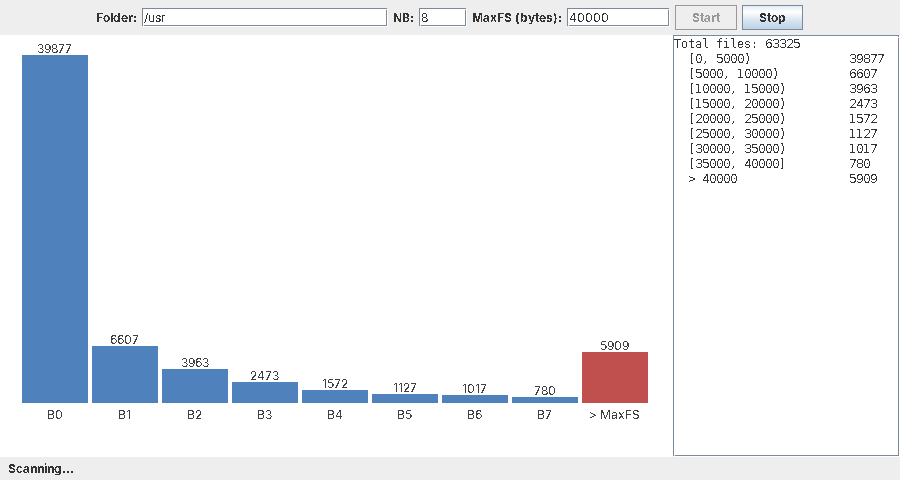
\includegraphics[width=0.82\textwidth]{gui.png}
\caption{The GUI (virtual-threads version) while scanning \code{/usr} with $NB=8$, $MaxFS=40000$.}
\label{fig:gui}
\end{figure}

\section{Comparison and verification}

\begin{table}[h]
\centering\small
\begin{tabularx}{\textwidth}{@{}lYYY@{}}
\toprule
 & \textbf{Event loop} & \textbf{Reactive} & \textbf{Virtual threads} \\
\midrule
Style & continuations on futures & declarative pipeline & imperative, blocking \\
Who waits for I/O & Vert.x worker pool; event loop never blocks & I/O scheduler threads & the virtual thread (unmounted) \\
Termination & \code{Future.all} composition & \code{flatMap} completion & recursive joins \\
Aggregation & merge in continuations (base), confined counters (ext.) & \code{reduce} / \code{scan} & local arrays + futures (base), monitor (ext.) \\
Shared state & none (thread confinement) & none (serialised signals) & none (base), lock-protected monitor (ext.) \\
Updates & periodic timer, event bus & stream + \code{sample} & notifier virtual thread \\
Stop & message, \code{stopped} flag, undeploy & \code{dispose()} & cooperative \code{Flag} \\
\bottomrule
\end{tabularx}
\caption{The three solutions side by side.}
\end{table}

The three versions were checked against an independent count (a Python script) on a synthetic tree
with files on the band boundaries ($0$, $MaxFS/NB$, $MaxFS$, $MaxFS+1$ bytes) and a symbolic link creating
a cycle, and on \code{/usr} (134\,929 files): all of them return exactly the same report.
Further checks: an unreadable sub-directory is skipped (run as a non-root user) and a FIFO is ignored; a non-existent
root, a file used as root and invalid parameters produce an error; in the interactive versions
stop, restart and completion were exercised repeatedly, verifying that no update is delivered after
the final outcome and that the scanning verticle undeploys itself.

\end{document}
